\documentclass[11pt]{article}

\usepackage{amsmath}
\usepackage{graphicx}
\usepackage{multicol}
\usepackage{natbib}
\usepackage{wrapfig}
\usepackage{hyperref}
\usepackage{tabularx}
\usepackage{setspace}
\usepackage{comment}
\usepackage{color}

\usepackage[compact]{titlesec}  
\titlespacing{\section}{0pt}{0pt}{0pt}
\titlespacing{\subsection}{0pt}{0pt}{0pt}
\titlespacing{\subsubsection}{0pt}{0pt}{0pt}

\oddsidemargin 0cm
\evensidemargin 0cm

\usepackage[margin=1in]{geometry}

\parindent 0cm
\parskip 0.5cm

\usepackage{fancyhdr}
\pagestyle{fancy}
\fancyhf{}
%\fancyhead[L]{AOSS Reference Sheet}
\fancyhead[C]{\small Full Lifecycle of Cyclones in the North Atlantic}
\fancyfoot[C]{Page \thepage}

\newcommand{\vb}{\mathbf}
\newcommand{\diff}[2]{\frac{d #1}{d #2}}
\newcommand{\diffsq}[2]{\frac{d^2 #1}{{d #2}^2}}
\newcommand{\pdiff}[2]{\frac{\partial #1}{\partial #2}}
\newcommand{\pdiffsq}[2]{\frac{\partial^2 #1}{{\partial #2}^2}}
\newcommand{\topic}{\textbf}
\newcommand{\arcsinh}{\mathrm{arcsinh}}
\newcommand{\arccosh}{\mathrm{arccosh}}
\newcommand{\arctanh}{\mathrm{arctanh}}

\begin{document}

\appendix

\addtocounter{section}{3}

\section*{Notes}

- African Easterly Waves
- Why does the number of cyclones decrease in the future?  Is this robust across models (but high resolution is needed)?  Humidity at 600hPa; shearing differences?  SST distribution?
- Focus on the northern Atlantic and eastern Pacific
- Why does intensity increase?
- Are coupled model simulations needed to assess tropical cyclones?  Coupled model biases are very problematic
- Extratropical cyclones and the tropical transition.  Is the tropical transition pushed farther North?  Detection algorithm based approach to ETCs.
- An outcome is a more robust detection / stitching algorithms
- Changes in landfall?  Assessment of regions which will be more susceptible to TC damage.  How does recurving affect this?
- "Changes in global circulation and the effect on local extremes"
- Leverage the ensemble of high resolution ensemble data
- Variable resolution over the Atlantic basin; run a bunch of ensembles at 25 km resolution
- What are the resolution dependencies of ETCs?
- Characterizing changing t-storms (size, wind speed, pressure, symmetry, latitude of max intensity, precipitation, latitude of maximum intensity, precipitation over land)
- Characterizing changing et-storms (size, wind speed, pressure, snow/rain precip. amounts, latitude of max. intensity)
 
\section{Project Description}

The next century will see unprecedented changes to the climate system.  These changes are particularly apparent to society through the behavior of extreme weather events. As stated in the third national climate assessment, ``changes in extreme weather and climate events, such as heat waves and droughts, are the primary way that most people experience climate change.''  Changes in such have been observed since at least 1950, and have been at least partially linked to climate change due to human influences (IPCC AR5 Synthesis Report).  In this manner, the characteristics of climate extremes are key indictors of climate change, and addressing observed and projected changes in these quantities will be crucial for future climate assessments.

This proposal will address the complete lifecycle of tropical cyclones in the North Atlantic basin:  Cyclogenesis, mid-life and termination.

The key scientific questions that are the focus of this proposal are as follows:
\begin{itemize}
\item[(Q1)] Is the location of tropical cyclogenesis in the North Atlantic basin modified under climate change in high-resolution climate model simulations?  {\color{red}[Bengtsson, Hodges and Roeckner (2006)]}  How does the projected intensification of the African Easterly Jet affect cyclogenesis off the African coast?

\item[(Q2)] How are the lifetime characteristics of tropical cyclones affected under future climate change in high-resolution climate model simulations?

\item[(Q3)] Why does the count of North Atlantic tropical cyclones decrease in future scenarios?
\end{itemize}

The central hypotheses of this proposal are as follows:

\vspace{-0.4cm}
\begin{itemize}
\item[(H1)] Changes in African Easterly Wave (AEW) activity is a driver for reduced tropical cyclone count and increased intensity in the North Atlantic basin.

\item[(H2)] The transition point for tropical cyclones to extratropical cyclones will be pushed north in response to increased carbon dioxide and/or increased sea surface temperatures.

\item[(H3)] The potential for landfall for cyclones in the North Atlantic will be pushed northward under future climate scenarios, increasing the vulnerability of the North American coastline.
\end{itemize}

The \textbf{uniting themes} of this proposal are \textbf{tropical cyclones}, \textbf{extratropical cyclones}, \textbf{climate change} and \textbf{big data}: This work will drive the introduction of a high-throughput cross-validated toolset for detecting and characterizing these atmospheric phenomena in large climate datasets.  Part of the uniqueness of this proposal is that it tackles scientific questions arising from tropical cyclones and extratropical cyclones within a unified framework by considering robust event detection methods as applied in the global context.  It further considers questions of attribution and prediction by leveraging these data analysis tools and large ensemble datasets to drive the most scientifically robust conclusions.

In addition to driving the development of new methods and tools, this proposal aims for several unique and novel results.  \textbf{High-resolution model simulations} will be a major focus of this work:  Under this study, it is hypothesized that high model resolution (here considered to be grid spacings less than 30 km) will greatly improve the simulation of AEWS, TCs and ETCs.  Further, it is anticipated that these features will be more realistic in the vicinity of rapidly changing topography, such as along the North American coast.  This proposal also aims to be the first to completely characterize the complete cyclone lifecycle in the \textbf{In the Community Atmosphere Model (CAM)} within the Community Earth System Model (CESM), verify that CAM5 produces a climatology consistent with observational data, and understand how the individual components of the cyclone will change under future warming scenarios.  Finally, in addition to their mean behavior, this proposal is also interested in studying the \textbf{variability} of these features by producing and leveraging access to large ensembles of model results.

The overarching objectives of the research component of this proposal are as follows: 

\begin{enumerate}
\item Develop robust methods for detection and classification of African easterly waves, tropical cyclones and extratropical cyclones, and provide improved tools for analysis of large climate datasets.

\item Characterize of the individual components of the cyclone lifecycle from genesis through extratropical transition or landfall in the North Atlantic at present and in the recent past.

\item Provide a scientifically and statistically robust risk assessment of projected human-induced climate change on tropical cyclones and extratropical cyclones.
\end{enumerate}

The remainder of this proposal is structured as follows: Motivation is presented in Section \ref{sec:Motivation}, background and ongoing work are presented in Section \ref{sec:BackgroundOngoingWork}, research milestone are presented in \ref{sec:ResearchMilestones}, and the timeline for the proposed work is presented in Section \ref{sec:Timeline}.

\subsection{Motivation} \label{sec:Motivation}

\subsubsection{Broader Impacts and Intellectual Merits}

\paragraph{Broader Impacts:}  

Landfalling TCs produce intense winds, heavy rain, high waves, and damaging storm surge in coastal locations \citep{EmanuelDivineWind}. They are currently estimated to be responsible for 19,000 fatalities per year and \$26 billion/year in damages worldwide \citep{Mendelsohn2012}, making them one of the most devastating natural phenomena. Furthermore, tropical cyclones are the costliest of all natural disasters in the United States\citep{Pielke1998}. Hurricane Katrina in 2005 caused at least \$100 billion in damages and about 1200 fatalities in the United States alone \citep{Blake2011}. More recently, Hurricane Sandy made landfall on the East Coast of the U.S. and, even though it was not classified as tropical at the time of landfall (having undergone extratropical transition), the cyclones' large size impacted a large swath of the coastline and urban areas making it the second-costliest cyclone after Katrina \citep{Blake2013}.  

Understanding how cyclones may change in the coming decades is of significant value to science and society. It can be expected that damages due to cyclone landfalls in the future will increase significantly due to growth of coastal population and property \citep{Pielke2008}. When put into context of a warming climate suggesting more intense tropical cyclones \citep{Knutson2010} understanding the changes cyclones is crucial for the United States, particularly North Atlantic cyclones. As global models continue to advance in both complexity and resolution the can provide necessary insight into projected changes in cyclone activity.  Such information will be valuable to society, contributing to informed decision making at the local and national level both in the public and private sectors.

\paragraph{Intellectual Merits:}  

The proposed research will make use of a series of ensemble high-resolution global model simulations to understand the impact of climate change on  North Atlantic cyclones. In particular the research will focus on the entire lifecycle of cyclones, from genesis to extratropical transition and/or landfall, using a novel TempestExtremes framework for event detection and tracking.  The work will provide new understandings into i) the impact of AEWs on TC formation in a warming world and ii) the effect of changes in TC characteristics due to climate change on extratropical transition and landfalling cyclones. Additionally, this project will support continued evaluation of high-resolution ($<$ 30 km) global models for the analysis of extreme weather events, such as tropical cyclones, as these next-generation models are a promising tool to understand the impact of anthropogenic climate change on extremes.  

\subsection{Strengths of the team}

The PI, Co-PI and their collaborating team are uniquely positioned to conduct multi-model ensemble intercomparisons, including variable-resolution configurations, of climate model output using a suite of cutting-edge atmospheric models and post-processing tools.

PI Kevin Reed brings considerable experience in high-resolution climate modeling.  His past research has focused on understanding the ability of the Community Atmosphere Model (CAM) to simulate tropical cyclones at present-day and next-generation horizontal resolution \citep{Reed2011a,Reed2011c,Reed2012b}.  This includes the study of how tropical cyclones and precipitation extremes change with climate change using decadal climate simulations at approximately 25-km horiztonal resoluton \citep{Wehner2014,Villarini2014,Wehner2015,Reed2015b}. Prof Reed also has developed techniques to utilize reduced complexity testbeds for understanding cloud, circulation and precipitation sensitivities in General Circulation Models (GCMs) \citep{Reed2012a,Reed2015a}. These simplified techniques have shown to be useful to rationalize robust behaviors of the Earth system and are vital to continued model development and intercomparison. Through his work, Prof. Reed has developed international collaborations in model development and high-resolution modeling.

This project will further benefit from Co-PI Ullrich's experience with atmospheric model development  (\cite{ullrich2010high, PHLPAURDN2011SPRINGER, ullrich2012operator, ullrich2012mcore, ullrich2014fluxform, guba2014viscosity, ullrich2014understanding, ullrich2014global}), numerical analysis (\cite{ullrich2011analysis, ullrich2012considerations}) and model evaluation (\cite{DCMIP2012TESTCASES, ullrich2014proposed, kent2013dynamical, ullrich2014baroclinic}).  PI Ullrich has been heavily involved with work on variable-resolution modeling \citep{zarzycki2014aquaplanet} and adaptive mesh refinement  \citep{collins2013nonhydrostatic, mccorquodale2014adaptive}. Many relevant tools have been developed by the Co-PI, including the SQuadGen grid generation tool (described in \cite{guba2014viscosity}), the TempestRemap post-processing toolkit \citep{ullrich2015remapping} and the TempestExtremes toolkit for extreme weather detection and characterization \citep{ullrich2015extremes}. He is heavily involved in national collaborations on climate projects, and is an organizer on a number of sessions and workshops which are related to atmospheric modeling. In addition, he is closely affiliated with ongoing climate research efforts at Lawrence Berkeley National Laboratory (LBNL) and the National Center for Atmospheric Research (NCAR).

\subsection{Background and Ongoing Work} \label{sec:BackgroundOngoingWork}

The focus of this proposal is on tropical and extratropical cyclones, which will be studied in the context of climate change and big data.  Of particular interest is the North Atlantic basin given the impact of cyclones on the U.S. and North America. Additional interest will be given to African easterly waves, as it is well known that they play a significant role in tropical cyclone formation in the North Atlantic. This proposal will bring together a number of existing technologies, datasets and studies in order to address its objectives, which are described below.

\subsubsection{African Easterly Waves}
African easterly waves are large-scale westward disturbances that originate over North Africa and are associated with the African easterly jet. These tropical waves typically have wavelengths of 2000-4000 km and time periods of 3-5 days \citep{Burpee1974,Reed1977}. African easterly waves are traditionally thought to develop by barotropic/baroclinic instability of the African easterily jet \citep{Burpee1972}, but recent research suggests that convection also plays an important role in the growth and development of the disturbances \citep{Hall2006,Thorncroft2008,Hsieh&Cook2005,Berry&Thorncroft2012}. African easterly waves are importance to the formation of tropical cyclones in the North Atlantic, with over 80$\%$ of major hurricanes in the basin originating from these waves \citep{Landsea1993}. Furthermore, Eastern Pacific Ocean tropical cyclone formation is also linked to African easterly waves \citep{Avila&Pasch1995}. 

A number of studies have explored African easterly wave activity in GCMs \citep{Ruit&DellAquila2010,Daloz2012,Skinner&Diffenbaugh2013,McCrary2014}. Recent work by \citet{Roberts2014} suggests that increased horizontal resolution improves the simulation of the tropical waves and therefore tropical cyclone counts in the North Atlantic.  Despite these studies, relatively little work has focused on the impact of climate change on the development and formation of African easterly waves and the connection to changes in tropical cyclones in the North Atlantic. Work by \citet{Skinner&Diffenbaugh2013}, using the CMIP5 dataset, indicates an increase in easterly wave strength (for those waves north of the African easterly jet), suggesting implications for the Atlantic Ocean basin. The proposed work will  further investigate how the African easterly wave activity behaves in higher resolution models in current and future climate, with the goal of understanding the impact of potential changes in African easterly wave activity on tropical cyclone in the North Atlantic.

\subsubsection{Tropical Cyclones}
Tropical cyclones (TCs) are extreme vortices that develop over the warm tropical oceans, and are among the most destructive geophysical phenomena. In the United States, tropical cyclones are the costliest of all natural disasters \citep{Pielke1998}. As a result, understanding how global and regional TC climatology will change in the coming decades is of significant value to society. Climate models are becoming a preferred tool to assess TCs in current and future climate conditions. Despite typical resolution limitations, it is well known that GCMs have the ability to simulate TCs, even at coarse horizontal resolutions of 100 km \citep{Knutson2010}. However, these simulated TCs are typically of weaker intensity and larger size than observed storms \citep{Walsh2007}. Using horizontal resolutions in the range of 10-30 km, more recent GCM studies have shown the ability to improve some of these resolution limitations \citep{Murakami2012,Manganello2012, Bacmeister2014, Wehner2014}

The general understanding is that global tropical cyclone frequency is likely to decrease, or remain relatively unchanged, with a likely increase in intensity under future climate scenarios (IPCC AR5 Synthesis Report). However, there is no consenus for the manner in which TC frequency and intensity will change regionally in a future climate using CMIP5 models \citep{Camargo2013}. The proposed research will study the attribution of anthropogenic climate change on TC intensity intensity, frequency and storm precipitation. Furthermore, the proposed work will address the questions of how climate change may impact TC characteristics, including genesis, in the North Atlantic basin by making use of ensemble simulations.  

\subsubsection{Extratropical Cyclones}

Extratropical cyclones are dominant features of the mid-latitude atmosphere associated with synoptic scale low pressure systems outside the tropics \citep{serreze1995climatological}.  Similar to tropical cyclones, these systems are responsible for high winds and extreme precipitation, and consequently have the potential for large socioeconomic impact \citep{ulbrich2009extra}.  Studies of extratropical cyclones under future climate scenarios suggest that the expansion of the Hadley circulation will drive extratropical cyclones poleward \citep{bengtsson2006storm} and the warmer climate will lead to an intensification of precipitation of these storms \citep{bengtsson2009will, zappa2013multi}.  {\color{red} Is there more literature on ETCs and climate change for frequency}. This proposal aims to address the question of changes in ETCs to anthropogenic forcing, with particular interest to those that originate from North Atlantic tropical cyclones through extratropical transition \citep{hart2001climatology}.  
%It will also address the issue of whether observed intensification over the southern hemisphere in reanalysis data is corroborated with model results, or is likely associated with an increase in the number of observing stations \citep{simmonds2000variability}.  Further, results from MERRA and C20C datasets (which have traditionally been neglected in favor of NCEP and ERA-40 data) will be integrated into the analysis.

\subsubsection{Global climate modeling with CESM} \label{sec:cesm-description}

The Community Earth-System Model (CESM) \citep{RBNetal2010NCAR} is a state-of-the-art Earth modeling framework developed at NCAR, consisting of atmospheric, oceanic, land and sea ice components.  This framework has been under development for nearly two decades, and has been used heavily in better understanding the effects of global climate change.  The atmopsheric component, CAM5, is further broken into two components: the dynamical core, which solves the 3D primitive equations of motion for the atmosphere, and the physics parameterization suite, which incorporates processes that occur on scales finer than the model grid scale. This project will utilize simulations from two different commonly used dynamics packages. The first package, the finite-volume (FV) dynamical core based on a regular latitude--longitude grid, is built upon a 2D shallow water approach described in \citet{Lin1996,Lin1997} and is mass-conservative in flux-form. The push for high-resolution climate simulations has required that CAM5 be sufficiently robust to operate on horizontal scales as fine as 10 km globally, although previous generations of the dynamical cores on latitude-longitude grid have been too slow at high resolutions to operate well at these scales.  This, in part, has led to the development of the CAM5 spectral element (SE) dynamical core \citep{dennis2012cam}, which utilizes a continuous fourth-order accurate Galerkin method on a highly scalable cubed-sphere mesh.  Current experiments are only now leading to the availability of CAM5 simulations on climate time-scales at 25 km global resolution \citep{Bacmeister2014, Wehner2014, Wehner2015, Reed2015b}.

It should be noted, that global modeling at these high is computational expensive.  The National Academy of Science report ``A national strategy for advancing climate modeling'' states: \textit{To enable higher resolution within computational constraints, alternative approaches such as regional climate models and global models with \textbf{variable-resolution, stretched grids or adaptive grids} have been developed to provide local refinements for geographic regions or processes of interest.}  In particular, recent advances in the SE dynamical core in CAM5 have focused on the development of variable-resolution capabilities as a means for better understanding interactions between the global and regional scale and to improve climate projections over a limited area, while reducing computational costs. The use of mesh refinement in the CAM5 framework is very recent, although early studies have suggested the usefulness of the configuration for studying regional climate impacts, including tropical cyclones \citep{Zarzycki2014multidecadal, Zarzycki2015clim}.

%As part of its objective, this proposal addresses the need for additional development and testing of these models for tackling real scientific problems.
\subsubsection{High-resolution CAM5 datasets} \label{sec:CAM-data} 

The proposed research will make use of numerous high-resolution CAM5 datasets already available through collaboration set forth by the PI and Co-PI. The first CAM5 set is the Climate Variability and Predictability (CLIVAR) Hurricane Working Group (HWG) experiments used to isolate changes in the climate system associated with accepted forcing mechanisms \citep{Wehner2015}.  Specifically, the experiments of interest for this proposal use present-day forcing which has been modified by (a) doubling atmospheric CO2 concentration (2xCO2), (b) increasing global sea-surface temperatures by 2 degrees (SST+2) or (c) a combination of (a) and (b).  CLIVAR runs have been completed using CAM5 over a 14-17 year integration period at 25 km with the FV dynamical core and are now available for analysis through collaborator Dr. Michael Wehner at LBNL.

Additional CAM5 configurations run by LBNL and NCAR will be utilized for this project. These simulations are run also run at 25 km horizontal grid spacing from 1980 through 2005 according to the observed Atmospheric Model Intercomparison Project (AMIP) protocols \citep{Gates1992,Gates1999} for surface temperatures, sea ice, ozone and greenhouse gases. The simulations are run with both dynamical cores discussed in Section \ref{sec:cesm-description}, but nearly identical physical parameterization suites \citep{RBNetal2010NCAR}. The CAM5-FV simulations have also been run by Dr. Michael Wehner as part of the CLIVAR HWG. In addition to the default simulation 26-year AMIP simulation 4 additional ensemble simulations have been perform for 1995 to 2005 with CAM5-FV. Additional CAM5 AMIP simulations with the SE dynamical core have been run as part of a larger group effort at NCAR under the direction of Dr. Julio Bacmeister (NCAR) to evaluate CAM5 at these high horizontal resolutions. In addition to to the AMIP-style simulation, the CAM5-SE simulations also include future time-slice experiment for 2070-2099 based on Representative Concentration Pathway (RCP) 8.5 to account for future greenhouse gas forcing. Finally, NCAR has recently completed a AMIP CAM5-FV ensemble simulation, with a different aerosol model configuration, for comparison to the CAM5-FV simulation run by LNBL.  In total, this proposed project would make use of 12 existing CAM5 high-resolution datasets for recent and future climate scenarios ranging from 11 to 26 simulation years each.  The list of simulations is summarized in Table \ref{t:runs}

\begin{table} 
\begin{center}
\caption{List of simulations.\label{t:runs} }
\ \\
\begin{tabular}{l c r l}
\textbf{Completed} \\
\hline
Configuration & Resolution & Length & Note \\ 
\hline
CLIVAR, CAM5-FV & 25 km & 14-17 years & 4 idealized climate forcings  \\
AMIP, CAM5-FV & 25 km & 26 years    & 2 full ensembles and  \\
& & & 4 11-year ensembles for 1995-2005 \\
AMIP, CAM5-SE & 25 km & 26 years    & \\
RCP8.5, CAM5-SE & 25 km & 30 years    & Time-slice 2070-2099 \\
\hline
\\
\textbf{Variable Resolution} & \textbf{To Be Completed} & & \\
\hline
Configuration & Resolution & Length & Note \\ 
\hline
AMIP, CAM5-SE & 100$\Rightarrow$25 km & 26 years    & 5 ensembles for 1980-2005 \\
RCP8.5, CAM5-SE & 100$\Rightarrow$25 km & 26 years    & 5 ensembles for 2070-2095 \\
\hline
\end{tabular}
\end{center}
\end{table}

In addition to the 12 completed runs by LBNL and NCAR, it is proposed that additional 10 additional CAM5-SE runs be used, 5 each for the AMIP and RCP 8.5 configurations.  These runs will use the variable-resolution configuration discussed in Section \ref{sec:cesm-description} with a 25-km high-resolution mesh over the North Atlantic ocean basin, similar to the setup in \citet{Zarzycki2014multidecadal}. Due to computational advantages, each variable-resolution simulation costs roughly 16\% of one globally uniform 25 km simulation.  Therefore, the 5 AMIP variable-resolution ensemble simulations will cost less than pre-existing global high-resolution CAM5-SE simulation. 

\begin{figure}[p]
\begin{center}
%\begin{tabular}{|p{4in}|}

\includegraphics[width=2.in]{NA_mesh.eps}
%\hline
%\end{tabular}
\end{center}
\caption{The proposed variable resolution mesh with 25 km grid-spacing over the North Atlantic and 100-km grid-spacing over the majority of the globe (from \citet{Zarzycki2014multidecadal}).} \label{fig:NA_mesh}
\end{figure}

\subsubsection{Justification for using CAM5 25 km to model Atlantic basin tropical cyclones}

CAM5 has shown an increasing ability to simulate tropical cyclones in the North Atlantic \citep{Wehner2014,Wehner2015,Reed2015b}.  Figure \ref{fig:NATCs} shows preliminary CAM5 tropical cyclone counts (e.g., all cyclones that reach tropical storm intensity or 17 m/s) in the North Atlantic using the two difference dynamical core configurations mentioned in Section \ref{sec:cesm-description}. When compared to observations from the International Best Track Archive for Climate Stewardship (IBTrACS, \citet{Knapp2010}) the CAM5 simulations produce between 2-3 less storms less per year for a 20-year period starting in 1980. Despite this slight bias in storm count, CAM5 does capture the interannual variability in the basin rather well, with correlations of 0.69 and 0.74 for CAM5-FV and CAM5-SE, respectively. These initial results, as well as the previous results, suggest that CAM5 is a good candidate to study the lifecycle of cyclones in the North Atlantic, as well as climate change impacts.

\begin{figure}[p]
\begin{center}
%\begin{tabular}{|p{4in}|}
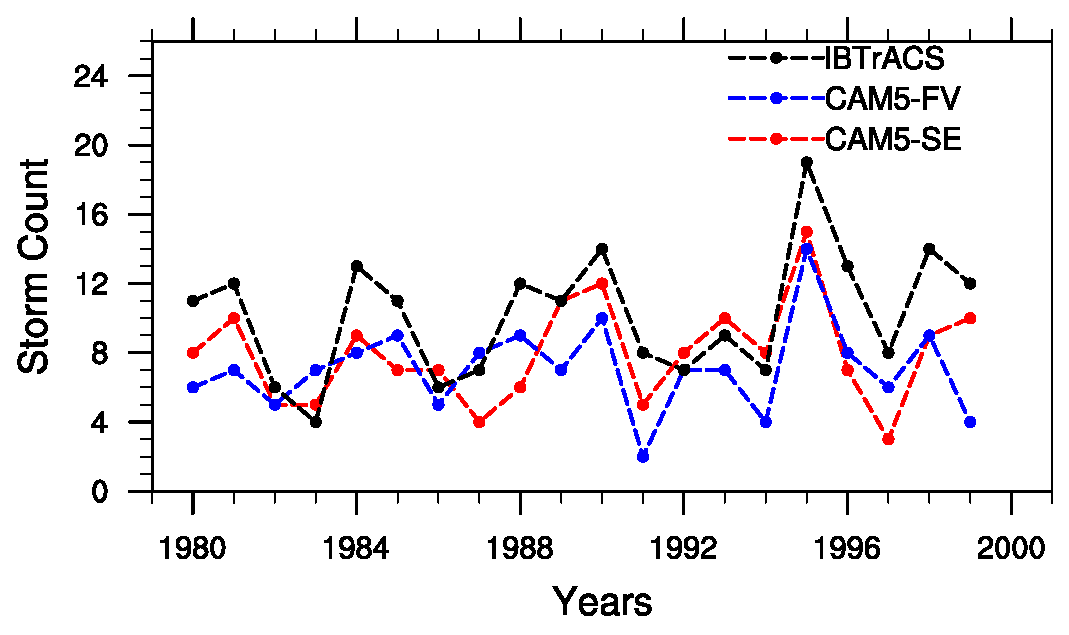
\includegraphics[width=5.5in]{NA_interannual.eps}
%\hline
%\end{tabular}
\end{center}
\caption{Annual counts of simulated high-resolution CAM5 and observed tropical cyclones from 1980 to 2000 in the North Atlantic ocean basin.} \label{fig:NATCs}
\end{figure}

\subsubsection{High-throughput event detection with TempestExtremes} \label{sec:TempestExtremes}

TempestExtremes software package, a new suite of flexible detection and characterization algorithms developed by the Co-PI for processing large climate datasets. This package uses an algorithmic framework known as ``MapReduce'' to first detect candidate events at individual times using specified criteria. Stitching is then used to track pointwise and areal detections in time. The result is a catalog of extreme weather events and associated characteristics whose generation can be automated and parallelized for multiple datasets.

\begin{figure}[p]
\begin{center}
%\begin{tabular}{|p{4in}|}
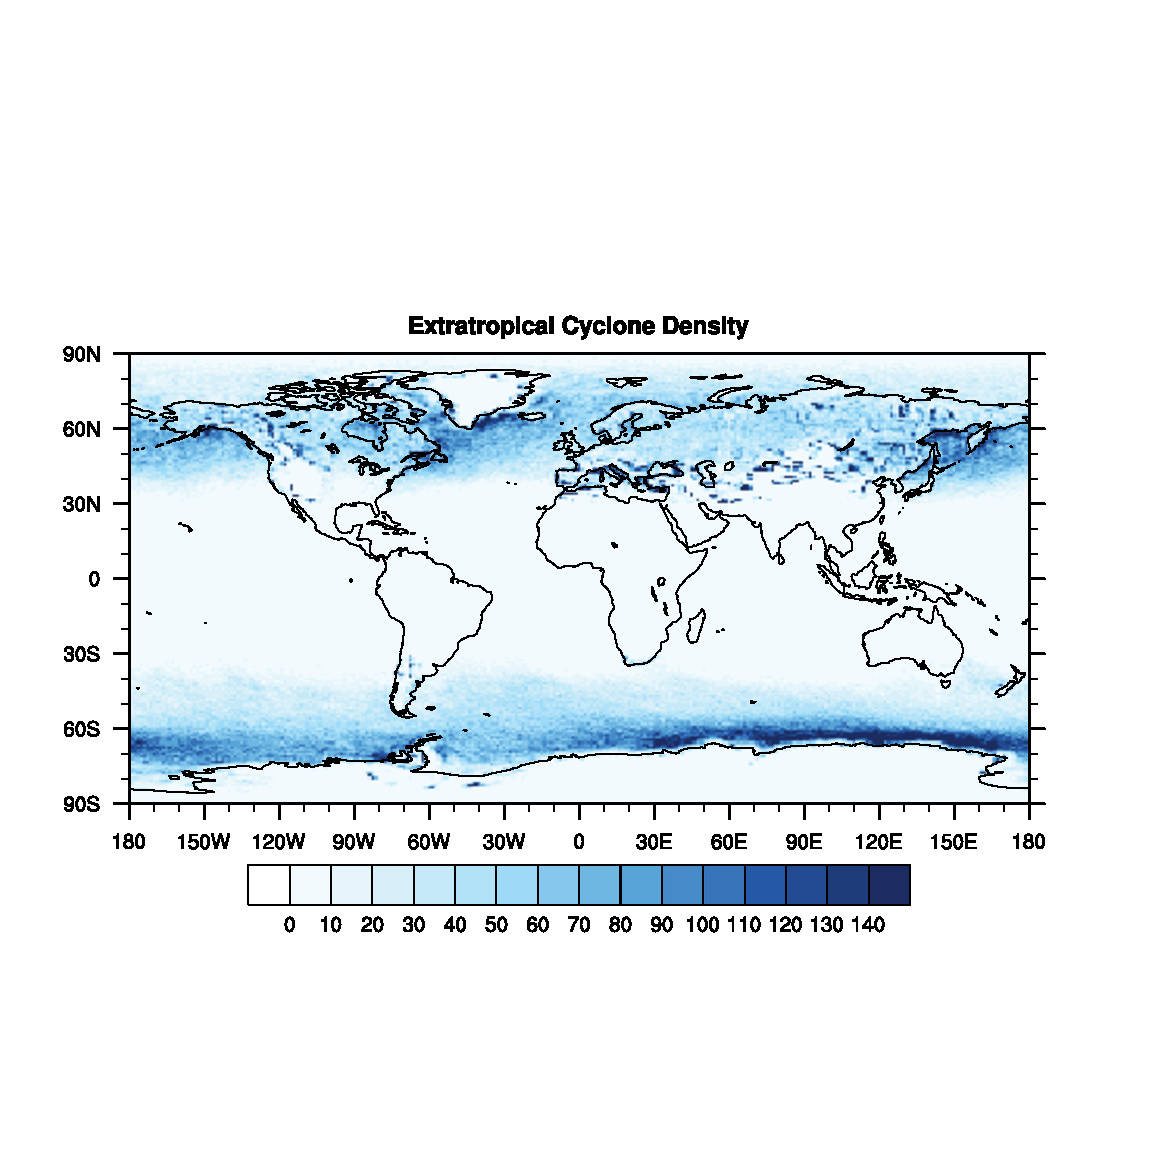
\includegraphics[trim=0.5cm 3.5cm 1cm 4.5cm, clip=true, width=4.5in]{density_plot}
\includegraphics[width=1.5in]{ETCChanges.png}
%\hline
%\end{tabular}
\end{center}
\caption{\textbf{(Left)} Example ETC counts from a 20-year CLIVAR climatological simulation, as obtained by selecting only pressure minima that (a) do not have an upper level warm core, (b) are within 4 degrees of a vorticity maximum, (c) are present over topography of maximum elevation 1500\ m, (d) are persistent for at least 2 days, (e) increase in pressure by  at least 0.1\ hPa over a distance of 1 degree in all directions, and (f) are in the latitude interval [90S, 20S] or [20N, 90N].  \textbf{(Right)} An example of differences between average annual ETC counts from a control simulation (climo) and a simulation with increased sea-surface temperatures (SSTplus2).} \label{fig:DensityPlot}
\end{figure}

In TempestExtremes, detection of both ETCs and TCs is handled by first searching for minima in the sea-level pressure field.  Thresholds can then be specified on the pointwise Laplacian of pressure, maximum or minimum latitude and topographic height at the point of detection.  Additional criteria are also available, including requirement or elimination of candidates based on the presence of a warm core aloft, the presence of a relative vorticity maximum, or the presence of a closed pressure contour.  Once candidate storms have been identified, stitching of candidates to form cyclone tracks is performed.  The stitching algorithm provides options for maximum distance between candidate points, minimum track duration, minimum distance between begin and endpoint, minimum path length, and other user-specified thresholds on quantities such as windspeed or surface pressure.  The stitching algorithm also provides an option for identifying trajectories with detection gaps, for example when candidates are present at times 1,2,3,5,6, and 7.  These criteria amalgamate a wide range of detection and stitching algorithms specified in the literature, including those criteria discussed above.  A plot of ETC densities for one possible configuration is depicted in Figure \ref{fig:DensityPlot}.  This proposal will apply this existing detection and stitching technology to the datasets in Section \ref{sec:Datasets} so as to isolate historical trends of North Atlantic cyclone characteristics, and improve statistical confidence in previously observed trends.

\subsubsection{Observation and Reanalysis products}\label{sec:Datasets}

{\color{red} Paul, I think the reanalysis is necessary for the ETCs and AEWs, modify as you see fit}

Reanalysis products represent climate model hindcasts which are tightly constrained to known observational data.  Development of these products has been a major research focus, particularly over the past decade, with more than half a dozen agencies now maintaining reanalysis datasets.  However, these datasets have the potential to differ significantly depending on the choice of model, specific model parameters, the number of observations and the methodology by which data is assimilated into the model.  Although several major reanalysis products are available, this proposal aims to focus on results from NCEP \citep{kalnay1996ncep}, ERA-40 \citep{uppala2005era}, ERA-Interim \citep{simmons2007era}, MERRA \citep{rienecker2011merra} and C20C \citep{compo2011twentieth}.  The use of multiple datasets is important for identifying and overcoming biases associated with specific atmospheric models that may contaminate the results \citep{jun2008spatial}, and will lead to a set of more robust scientific conclusions. For tropical cyclones, observations from the International Best Track Archive for Climate Stewardship (IBTrACS, \citet{Knapp2010}) for the same time period (1980-2005) will be used. The dataset, endorsed by the World Meteorological Organization, merges tropical cyclone information, including tracks and intensity, from numerous international meteorological centers into a single dataset.

\subsection{Research Milestones} \label{sec:ResearchMilestones}

The research milestone will be approached in a step-by-step manner as described in the following sections. A set of relevant scientific questions are also provided that will be addressed by the proposed research. All task will incorporate both aspects of validation with present-day climatology and future climatology. When combined, the tasks will provided a novel approach to characterize the representation of the entire lifecycle of North Atlantic cyclones in current and future CAM5 simulations, helping to answers important questions as to how anthropogenic climate change will impact relevant societies in the region.

\subsubsection{Task 0: Validate Cyclone Detection and Characterization Framework}

 {\color{red} I'm thinking we drop this section as most of everything states has been stated in the previous Section or will be reiterated in the other Tasks. Thoughts? }

The first objective of the proposed research will be to develop a robust tracker, TempestExtremes, for high-resolution climate model output. The tracker would allow for seamless tracking of the entire lifecycle of cyclones in the North Atlantic. Previous work has demonstrated that the TempestExtremes framework to be successful in tracking ETCs as shown in Section \ref{sec:TempestExtremes}. This makes TempestExtremes an attractive framework to straightforwardly expand the detection algorithm to included TCs, therefore making the tracking of TCs through extratropical transition feasible within a single framework. To complete cyclone lifecycle the TempestExtremes framework will also need to incorporate detection of the origins of the tropical cyclone, particularly those that develop from AEWs. {\color{red} Need to say a little more on AEW tracking, TCs detection is straightforward}.

Following the further development cyclone TempestExtremes framework, the algorithm will be applied to the series of the present-day AMIP CAM-FV simulation. This model dataset is choose for the validation process as it has already been well study in its ability to simulate TCs \citep{Bacmeister2014,Wehner2014} and is readily available to community. While particular interest for this proposal is to investigate the lifecycle of cyclones in the North Atlantic, the TC component of the framework will be applied to the entire global dataset to ensure the validity of the framework in all ocean basins. For the validation observations described in Section ~ref{sec:Datasets} will be used to evaluate the detection of ETCs, TC and AEWS.  This will include the use of the  from the IBTrACS and reanalysis datasets for the same time period (1980-2005). The comparison will help understand biases in tropical cyclone global distribution, genesis location and intensity worldwide.

\subsubsection{Task 1: African Easterly Waves and Cyclogenesis} 

This task investigates the effect of climate change on the behavior of cyclogenesis in the Atlantic basin.  Preliminary work has shown a noticeable decrease in the formation of tropical cyclones in the North Atlantic in the CAM5-SE simulations. {\color{red} Need to run tracker on RCP 8.5 setup soon}. Figure \ref{fig-rcp}, shows the track density of TCs for present-day and future simulations using the TC detection algorithm and tracker utilized for this analysis is that used and described in \citet{Zhao2009}. The figure indicates a decrease in TCs basin-wide with the largest decrease in the eastern part of the basin off the coast of Africa. The track densities are calculated similar to \citet{Done2013} and is defined as the number of TC genesis points or tracks within a 5 degree radius of a given point per year. This pattern suggests that there is some connection between the future distribution and African Easterly Waves.  Specifically, we will address the following question:

\textit{Can the modeled decrease in North Atlantic basin tropical cyclone counts be attributed to a decrease in tropical cyclone initiating African Easterly Waves?}

Using the seamless detection algorithm described in Task 1, the relationship between AEWs and TCs will be explored both in the idealized CLIVAR experiments and AMIP simulations using the ensemble variable resolution simulations. In particular, the location and intensity of AEWs will be investigated, as well as the efficiency of the tropical waves to develop into TCs.  Furthermore, a comprehensive investigation of other environmental factors, including shear, will be pursued. Changes to the African Easterly Jet As pointed out by \cite{skinner2013contribution}, increased regional temperature gradients and intensification in the strength of convergence and uplift along the Intertropical Front of Africa may lead to an increase in the strength of AEWs.  However, it remains unclear how the frequency of AEWs, and particularly tropical cyclone initiating AEWs will be affected under future climate.

To address this question, we propose to implement AEW tracking capability in TempestExtremes.  Detection and tracking of AEWs has been historically performed using either meridional velocity \citep{Burpee1974, Reed1977} or vorticity \citep{hodges1995feature, thorncroft2001african} at the 850 hPa or 600 hPa level.  We will implement both tracking techniques in TempestExtremes, and will further investigate the use of sea-level pressure minima as an alternative tracking strategy.  The tracking algorithm will be limited to the region $[5^\circ N, 25^\circ N]$ and $[5^\circ W, 35^\circ W]$ in order to prevent spurious detection of non-AEW activity.  In conjunction with the TC detection scheme described in Section \ref{sec:TempestExtremes}, this approach will allow us to identify TC precursors in the form of AEWs and determine what role the strength of AEWs plays in triggering cyclogenesis.  As pointed out by \cite{thorncroft2001african}, AEWs from the southern side of the AEJ play a much greater role in cyclogenesis than AEWs on the poleward side.  Consequently, we will also track the position of the AEJ and determine if our model simulations show any trend in the mean latitudinal position of the jet that may affect the trajectory of AEWs.

%\cite{hodges1995feature} identifies a technique for tracking AEWs in terms of the vorticity.

%\cite{thorncroft2001african} argue that AEWs on the southern side of the AEJ play a much greater role in tropical cyclogenesis than AEWs on the poleward side.  ``This result suggests that Atlantic tropical cyclone activity may be influenced by the number of AEWs leaving the West African coast, which have significant low-level amplitudes, and not simply by the total number of AEWs.''

%Following \cite{thorncroft2001african}, AEWs will be investigate over the latitudinal range $[5^\circ N, 15^\circ N]$ and $[5^\circ W, 25^\circ W]$.

%: ``We find that increases in regional temperature gradients and the strength of convergence and uplift along the Intertropical Front of Africa lead to increases in the strength of AEWs.''  

%\cite{skinner2012african}: ``Given favorable conditions for cyclogenesis in the eastern Atlantic, AEWs, particularly those associated with convection over West Africa, develop into tropical cyclones.''

%Indeed, nearly all models simulate an increase in the occurrence of intense and extremely intense AEWs along the Sahel?Sahara border (Fig. 5). This includes median changes of +2.0 events per season (and +39\%) for intense AEWs, and +0.8 events per season (and +72\%) for extremely intense AEWs.

\subsubsection{Task 2: Tropical Cyclone Tracks, Intensity and other Characteristics}

This objective studies the effect of climate change on the characteristics of North Atlantic TCs during their lifetime. Previous work by \citet{Wehner2015} using the high-resolution CAM5 CLIVAR simulations suggests an global decreased TC frequency under the idealized warming forcings. The results also suggest an increase in intense TCs, an increased average storm duration and a poleward in genesis and track densities in the warmer scenarios. However, this CAM5 analysis was not performed at the basin level, specifically the North Atlantic. Understanding how the characteristics of TCs in the North Atlantic will change in the coming century is critical to coastal communities and the U.S. as a whole. Preliminary, CAM5-SE results (see Fig. \ref{fig-rcp}) do suggest that there is a decrease in North Atlantic storms. While numerous studied have investigate the impact of enhanced greenhouse gas forcing {\color{red}Will add citations}, such studies have typical be performed with nest-regional models and/or at lower horizontal resolutions than the 25 km grid spacings proposed here.  

\emph{Do North Atlantic tropical cyclones exhibit similar changes in storm characteristics (intensity, duration, distribution etc.) as seen in the global response to the idealized forcings?}

Previous studies of TCs at high-resolution in climate models are typically limited to one realization (i.e. one ensemble member). As mention in Section \ref{sec:CAM-data}, only recently have ensemble simulations been completed in the CAM5-FV AMIP configuration for the period of 1995 to 2005 in collaboration with Michael Wehner at LBNL. In addition, with the proposed CAM5-SE AMIP and RCP 8.5 ensemble simulations offer a unique opportunity to study changes North Atlantic tropical cyclone climatology. Utilizing the enhanced TempestExtreme framework the characteristics of TCs will be explored in the various CAM5 configurations. Making use of such a large high-resolution ensemble will allow for a robust analysis of the impact of a warming climate on North Atlantic TC intensity, track duration and track distribution. Such an analysis is truly novel for CAM5 at these resolutions.

{\color{red} I am thinking about adding TC size as a new metric and adding this in the hypothesis: Size will increase}

%In addition, the North Atlantic changes can be put into the context of the CAM5-FV CLIVAR simulations with idealized forcings, which present a different form of unforced variability given that the sea surface temperature is the same from year to year. In the AMIP ensemble simulations are mos
 
\subsubsection{Task 3: Characterization of the Extratropical Transition}

The extratropical transition of tropical cyclones is an important meteorological phenomenon whereby warm-core tropical cyclones transition into cold-core ETCs when they are sufficiently far from the tropics.  The extratropical transition has been studied in detail in the meteorological literature, and is fairly well understood \citep{hart2001climatology}.  However, the extratropical transition has not been thoroughly studied in the context of climate change.  In particular, studies on the effects of future climate have largely suggested that tropical cyclones will generally be fewer in number but will generally be more intense \citep{Knutson2010}, whereas many past studies of ETCs have agreed that although ETCs will be fewer in number, only precipitation intensity is expected to increase \citep{bengtsson2009will}.  Consequently, it is worthwhile to examine the influence of the changing climate on ETCs which occur due to extratropical transition of tropical cyclones in the North Atlantic using the infrastructure developed as part of this proposal.

\emph{Is there a shift in the location and frequency of extratropical transition of North Atlantic cyclones in the future?}

TempestExtremes offers the unique ability to track tropical cyclones and extratropical cyclones under one framework, and as a result the ability to capture cyclones that undergo extratropical transition in the North Atlantic basin.  TempestExtremes has been shown to be reliable in detecting and tracking extratropical cyclones (see Fig. \ref{fig:DensityPlot}) and this work will characterize the ETCs that originate form the transition of tropical cyclones. The process of extratropical transition has not previously been studied in the CAM5 context as high-resolution simulations are required to capture the precursor tropical cyclones. Therefore, the proposed worked will extensively investigate the number of tropical cyclones that undergo extratropical transition, as well as the intensity, location and distribution of such cyclones.  

In order to perform such an analysis, the proposed ensemble CAM5 CLIVAR and AMIP simulations will be crucial.  Particularly, observation indicate that on average 46$\%$ of tropical cyclones undergo extratropical transition in the North Atlantic \citep{hart2001climatology}. Given the relatively low number of North Atlantic tropical cyclones in observations and CAM5 and therefore the expected even lower number of cyclones undergoing extratropical cyclones, the ensembles will provide for more robust statistics. This will be necessary for characterizing the full lifecycle of cyclones in the North Atlantic. 

While previous work has studied extensively potential changes in tropical cyclones and extratropical cyclones in the North Atlantic under future radiative forcing, little is known to how the process of extratropical transition will be altered. Recent events, including Hurricane Sandy, have brought a renewed interest into extratropical transition and the devastating impacts that transitioning cyclones can have on the East Coast of the United States \citep{Blake2013}. As stated, previous and preliminary work with CAM5 has indicated that the number of tropical cyclones in the North Atlantic will decrease under future warming scenarios. This may suggest a decrease in the number of TCs that undergo extratropical transition.  However, \citet{Wehner2015} suggests that due to warmer sea surface temperature the duration of TCs increased globally in the CAM5 CLIVAR simulations, indicating that the ability of TCs to reach regions where extratropical transition occurs may increase.

The proposed work will shed new light on this subject area by making use of the CAM5 ensemble simulations for both present day and future climate forcing. Combined with the previous task for TCs, the proposed work will qualify future trends in tropical cyclone intensity, tracks and duration and the implications of such trends for extratropical transition in the North Atlantic.

\subsubsection{Task 4: Characterization of Landfalling Cyclones}

{\color{red}[Still working on this section - Add anything if you have ideas]}

Landfalling storms cause the most direct impact on the United States and other North American countries.  In particular, landfalling tropical cyclone cause .... in damage in the United States alone. A disproportion of the damage coming from individual storms that are particularly intense or that impact vulnerable regions.  {\color{red}[More motivation]}

\emph{The there increased potential for North Atlantic cyclones to make landfall further north?}

By using the unified TempestExtreme framework for cyclones in the North Atlantic, the research will enable a detailed investigation of landfalling cyclones.  This will include landfalling tropical cyclones, extratropical transitioning tropical cyclones and extratropical cyclones that have fully transitioned from tropical storms. This task will incorporate the analysis of all of the previous tasks. Utilizing the CAM5 ensemble simulations the analysis will include diagnosing changes in the frequency, spatial distribution, intensity and size of landfalling cyclones in the future climate scenario.  Furthermore, the study will investigate wether there are changes in the frequency of transition storms that can also have significant impacts on coastal communities.

This investigation will benefit from previous research that has studied the climatology of landfalling tropical cyclones and the associated precipitation. But by incorporating storms that are undergoing extratropical transition, the research will offer new insights into the full range of potential climate impacts of cyclones in the North Atlantic. 

\subsection{Online access to climate data and results}

Dissemination of climate data and scientific results is an important issue for increasing public understanding of climate change.  To this end, the co-PI will work to develop a website (via the domain \url{http://climate.ucdavis.edu}) which allows for easy access to the results of the research component of this proposal, as well as other results that draw from existing climate data.  This webspace would allow for users to query the database of climate data, and would provide frequent and accessible commentary on the latest results to emerge from the climate science community.  The co-PI's past experience as a professional web developer and experience with HTML and PHP will be advantageous to the development of this project.

\subsection{Timeline} \label{sec:Timeline}

{\color{red}[Still working on this section - Add anything if you have ideas]}

Each of the graduate student researchers involved in this project will work on various component of the cyclone lifecycle presented in this proposal: either TC genesis through AEWS or TC termination through landfall or extratropical transition. It is anticipated that there will be substantial collaboration in integrating the total lifecycle of cyclones in the North Atlantic and on the technical level.  Each year of the proposal is expected to be approximately associated with two tasks as described in Section \ref{sec:ResearchMilestones}.  The approximate timeline is as follows:

\begin{tabularx}{\textwidth}{cX}
\hline
\textbf{Year 1} & $\cdot$ Further validate and test cyclone detection framework. \\
& $\cdot$ Begin validation of framework on CAM5-FV model dataset.  \\
& $\cdot$ Setup and start CAM5-SE present-day and RCP8.5 variable resolution ensemble runs. \\
\hline
\textbf{Year 2} & $\cdot$ Finalize framework validation using CAM5-FV. \\
& $\cdot$ Write overview article introducing lifecycle detection framework .\\
& $\cdot$ Complete CAM5-SE present-day and RCP8.5 variable resolution ensemble runs. \\
& $\cdot$ Complete analysis on varibility using CAM5-FV and CAM5-SE ensemble simulations. \\
\hline
\textbf{Year 3} & $\cdot$ Write journal article on North Atlantic cyclone variability. \\
& $\cdot$ Complete analysis of future climate simulations. \\
& $\cdot$ Write journal article on North Atlantic cyclone activity in future climate. \\
\hline
\end{tabularx}

We anticipate that multiple major peer-reviewed publications will arise from this work, addressing the studies of detection, attribution and prediction. Further, this work will be presented at major scientific meetings, including the annual meetings for the American Meteorological Society, the European Geophysical Union and the American Geophysical Union.

{\setbox0\vbox{\bibliography{NSFCyclones-Bibliography}}}
\bibliographystyle{wileyqj}

\end{document}
